%%%%%%%%%%%%%%%%%%%%%%%%%%%%%%%%%%%%%%%%%%%%%%%%%
%------ LaTeX-Template für Abschlussarbeiten, Prof. Thomas Görne, Dezember 2012 --------
%------ Modified by B.Sc. Julius Neudecker, May 2021 ------
%%%%%%%%%%%%%%%%%%%%%%%%%%%%%%%%%%%%%%%%%%%%%%%%%

%---- Header (mit Formateinstellugen) laden, Inputencoding prxfen ------

%%%%%%%%%%%%%%%%%%%%%%%%%%%%%%%%%%%%%%%%%%%%%%%%%
%---- LaTeX-Header fuer Abschlussarbeiten, Prof. Thomas Goerne, Dez. 2012/Aug. 2013 ----
%------ Modified by B.Sc. Julius Neudecker, May 2021 ------
%%%%%%%%%%%%%%%%%%%%%%%%%%%%%%%%%%%%%%%%%%%%%%%%%

\documentclass[12pt,paper=A4,pointlessnumbers,bibtotoc,liststotoc,DIV=11,BCOR=1mm]{scrreprt}
% BCOR ist die Bindekorrektur (verlorener Rand am linken Blattrand)! Wert haengt von der Art der Heftung ab!!
% DIV ist eine Satzspiegeleinstellung von KOMA-Script / sccreprt.

\pagestyle{headings}

\usepackage[T1]{fontenc} % Font Encoding fuer europaeische Schriften mit Umlauten (Unterstuetzung der Worttrennung)
\usepackage{lmodern} % PostScript-Varianten der TeX Computer Modern-Schriften laden
\usepackage[english]{babel} % Spracheinstellungen fuer Englisch und Neudeutsch laden

\usepackage{graphicx} % Grafikeinbindung (fuer .JPG, .JPEG, .PNG und .PDF, falls pdflatex benutzt wird)
\usepackage[table]{xcolor} % ermoeglicht farbige Schrift und farbige Tabellenzeilen
\definecolor{black}{gray}{0} % Umdefinition der Farbe black, falls noetig (0=schwarz, 1=weiss)
\definecolor{dblue}{rgb}{0.1,0.2,0.6} % Dunkelblau, fuer Hyperlinks
\definecolor{lgray}{gray}{0.9} % Hellgrau, fuer Tabellen (0=schwarz, 1=weiss)

\usepackage{booktabs} % fuer schoene Tabellen

\usepackage[round,authoryear]{natbib} % Literaturverweise mit Name/Jahreszahl in runden Klammern
\bibpunct[:\,]{(}{)}{,}{a}{}{,~}  % Feinformatierung der Natbib-Zitierweise

\usepackage[hyphens]{url}
\usepackage[colorlinks=true,linkcolor=black,citecolor=dblue,urlcolor=dblue]{hyperref} 
\usepackage{hyperref}  
% die Pakete url und hyperref ermoeglichen anklickbare URLs im Quellenverzeichnis in definierter Farbe, 
% sie ermoeglichen den Zeilenumbruch bei langen URLs, und sie erzeugen Hyperlinks (Farbe s.o.) 
% zwischen Quellenverweis und Quellenverzeichnis sowie zwischen label und ref im PDF-Dokument

% Fonteinstellungen fuer Bildunterschriften: Unterschrift serifenlos, "Abbildung" fett (bfseries = bold face series)
\setkomafont{captionlabel}{\sffamily\bfseries}
\setkomafont{caption}{\sffamily}

% Ordner für Grafiken
\graphicspath{ {./images/} }

%% ToDo Notes
\newcommand\todo[1]{\textcolor{red}{#1}}

%------------------------------------------------------------------------------------------------------------------
%------ Eigenstaendigkeitserklaerung im gerahmten Kasten (parbox in einer framebox) ------
%------------------------------------------------------------------------------------------------------------------

\newcommand{\eigen}{
\setlength{\fboxsep}{2ex}
\setlength{\fboxrule}{0.8pt} 
% Einstellungen fuer Rahmenabstand und Rahmendicke der Framebox
\begin{center}
	\fbox{
		\parbox{0.8\linewidth}{
			I hereby confirm that this thesis is my own work and that I have not sought or used inadmissible help of third parties to produce this work and that I have clearly referenced all sources used in this thesis. I have fully referenced and used inverted commas for all text directly or indirectly quoted from a source.
		\par\bigskip\bigskip\bigskip\bigskip
		\hspace*{0.8cm}Place and date \hfill \vorname~\nachname\hspace*{0.8cm}
		}
	}
\end{center}
}

%%%%%%%%%%%%%%%%%%%%%%%%%%%%%%%%%%%%%%%%%%%%%%%%%

\usepackage[utf8]{inputenc} % Inputencoding, universell

%------------------------ Titelblatt-Layout laden ----------------------------------

%%%%%%%%%%%%%%%%%%%%%%%%%%%%%%%%%%%%%%%%%%%%%%%%%
%------ LaTeX-Titelblatt fuer Bachelorarbeiten, Prof. Thomas Goerne, Dezember 2012 -------
%------------------------------------------------------------------------------------------------------------------
%--------------------------------- Deklarationen fuer die Titelseite  --------------------------------------
%%%%%%%%%%%%%%%%%%%%%%%%%%%%%%%%%%%%%%%%%%%%%%%%%

\title{\titel\\[2ex]
\LARGE Masters Thesis\\
\large To obtain the academic degree M.Sc.\\[1.5ex]
\LARGE \vorname~\nachname\\[0.5ex] 
\large \matrikelnummer
}

\author{\unitlength1mm
\large\raisebox{-1ex}{
\includegraphics[width=4em]{HAW_wuerfel}}\hspace{1ex}
\parbox[b]{11.2cm}{\sffamily\large%
University of applied sciences Hamburg\\[-0.2ex]
Faculty of Design, Media und Information\\[-0.2ex]
Department of Media Engineering
}\\[6ex]
\sffamily\large First examiner: \erstpruef\\[0.5ex]
\sffamily\large Second examiner: \zweitpruef}

%%%%%%%%%%%%%%%%%%%%%%%%%%%%%%%%%%%%%%%%%%%%%%%%%

%---------------------------- Titeldefinitionen --------------------------------------

\newcommand{\vorname}{Julius}
\newcommand{\nachname}{Neudecker}
\newcommand{\matrikelnummer}{2025850}

\newcommand{\titel}{{[Working Title] Using a neural interface for interaction in virtual reality}\\[0.2ex] 
				\Large an HCI study}

\newcommand{\erstpruef}{Prof. Dr.Roland Greule}
\newcommand{\zweitpruef}{Dipl. Inf. Rüdiger Höfert}

\date{preliminary version from \today}   % praktisch fxr Vorab-Versionen. 
%\date{\sffamily Hamburg, 30.06.2021}  % Abgabedatum!

%--------------------------------------------------------------------------------------
%----------------------------- hier gehts los! --------------------------------------
%--------------------------------------------------------------------------------------

\begin{document}
    \selectlanguage{english}
    \maketitle
    \tableofcontents
    \clearpage          % Seitenumbruch

    %------------ Zusammenfassung / Abstract ------------------

    \thispagestyle{empty}
    \selectlanguage{english}
    \section*{\centering\abstractname}
    Modern technology evolved to pick up the eletric signals emitted from the human brain in order to generate user input to eletronic equipment. This study aims to evaluate a demo use-case by using a neural interface from nextmind to control user interactions in Virtual Reality.

    % --- Julius Text Sections ---

    \chapter{Introduction}

        %what is it
        %why does it make sense
        %what is the market evaluation


        In recent years significant progress has been made on the development of interfaces which relies on direct interaction with the brain itself. \todo{find some sources} The latest popular example is \textit{Neuralink} with their monkey learning to play the game \textit{Pong} only by using its brain (\cite{Neuralink.2021}). However there are more examples of a working interface: \todo{Do som research here}.
        These interfaces are generally called \textit{Brain-Computer-Interface} or \textit{BCI} in short. The general working principle is sensing the electrical signals of the brain and use this information to generate any kind of arbitrary output \todo{find source}. 
        In certain use cases like motoric reactions to visual cues, this could potentially reduce total reaction time. This study aims to examine a potential use case with a device which is readily available to consumers.
        

        \section{Brain-Computer-Interfaces}

            In this section a general overview of the working principle of these interfaces will be provided. Since this study is aimed at computer science and HCI\footnote{Human Computer Interaction}, the neuroscience and medical domain will be only covered very briefly.

            \subsection{Interfacing with the brain}

                %https://www.frontiersin.org/articles/10.3389/fnins.2016.00295/full

                First studies began by \cite{Vidal.1973}, who investigated the possibility to use EEG\footnote{Electroencephalogram} waves, which were first recorded by \cite{Berger.1929}, as a way to create a direct interaction between a machine and a human brain. 

                There are three types of BCIs: invasive, partially invasive and non invasive. This depicts the degree of intrusion into the skull and brain tissue. \textit{Invasive} BCIs are electrodes, which are implanted directly into or onto the grey matter of the brain. This can cause long term issues like scars and also degraded singal strength according to \cite{Abdulkader.2015}. 
                Partially invasive BCI however are although located within the skull not in direct contact with the grey matter.
                Non-Invasive BCI are only placed on the head without intrusion of any tissue.
                Due to the direct contact, invasive BCI provide the best resolution of the measured signals. Non-invasive BCI in comparison suffer from signal degradation and deformation of the cranial bone tissue. 
                Therefore partially invasive BCI are a compromise between signal strength and induced medical conditions.

                The way these interfaces work is based on the same principle: A human brain emits electrical signals, which can be picked up.
                According to \cite{Vidal.1973}, they can be described as follows:

                \medskip
                \emph{"Embedded in this sustained "spontaneous" or "ongoing" electrical activity, short, distinctive (0.5-2 sec) waveforms can be found that are evoked, for instance, when a brief sensory message (stimulus) such as a brief illumination of the visual field or a tap on the forearm is received by the subject."}
                \medskip

                Based on the region of the brain, where these originated, they can be correlated to certain stimuli or mental and emotional states (\cite{JardimGoncalves.2018}).

            \begin{itemize}
                \item Picking up brain activity
                \item Usage for interacting with eletronic equipment
            \end{itemize}

        \section{Related work}

            Whats state of the art, what has been done so far in research and where is my study in context?

            \begin{itemize}
                \item State of research
                \item Applications in the medical domain
                \item Applications in the HCI domain
                \item other...
            \end{itemize}

        \section{Use case "Neural Interface in VR"}

            % NextMind -> Proprietary
            % Best Guess: VEP – visuell evozierte Potentiale ermöglichen eine Beurteilung des Sehnerven
            % und der Sehbahn, sie werden über der Sehrinde im okzipitalen Kortex abgeleitet.

            I don't have a certain use-case in mind at this stage. Therefore this section is still very generic at the moment.

            \begin{itemize}
                \item Use Case description
                \item Research goals
            \end{itemize}        

        \section{Hypothesis}

            \begin{itemize}
                \item definition of research goals
                \item hypothesis
            \end{itemize}

    \chapter{Technological challenges}

        Due to being non-invasive there must exist certain drawbacks with this technology. I want to examine the shortcomings and possible ways to overcome these.    
        A valuable resource of information might be nextminds homepage \cite{NextMind.}.

        \section{Resolution of the Interface}

            \begin{itemize}
                \item definition of the resolution parameter
                \item input taxonomy diagram
                \item how to examine with survey                                     
            \end{itemize}

        \section{Constraints}

            As far as I understood, the interface allows for four different interaction goals. It would be interesting to see, which kinds of interaction are possible.                

            \begin{itemize}
                \item Interaction objects
                \item interaction types in regard to input taxonomy
                \item evaluation in user survey
            \end{itemize}

    \chapter{Survey Structure and layout}

        \section{Considerations}

            \begin{itemize}
                \item Which topics do I want to evaluate in detail
                \item what are my tools
                \item Who is my audience
                \item how to I operationalize the values for context
                \item What are my performance indicators
            \end{itemize}

        \section{Survey structure}

            Based on the findings, I want to define the survey in this section.

            \begin{itemize}
                \item item 1
                \item ...
            \end{itemize}

        \section{Survey}

            How is the survey carried out. This depends largely on the outcome of section survey structure.

            \begin{itemize}
                \item item 1
                \item ...
            \end{itemize}

    \chapter{Survey results}

        Once the study has been structured and carried out, I can write down the results.

    \chapter{Findings}

        This section also depends on the outcomes in context to the resarch question.

    \chapter{Conclusion}

        \section{Results}

            Summarizing the results and findings of the study briefly.

        \section{Future Work}

            Based on the findings and new devices on the horizon, this should give a brief outlook on how to continue this research.

    \chapter{Acknowledgements}

        ...


    % --- /Julius Text Sections ---

    %--------------------------- Text -------------------------------

    \chapter{Mathestuff}

        \section{Pictures}

            %----------- BILD ANFANG -------------
            \begin{figure}[htp]     % h=here, t=top, b=bottom, p=page
                \centering
                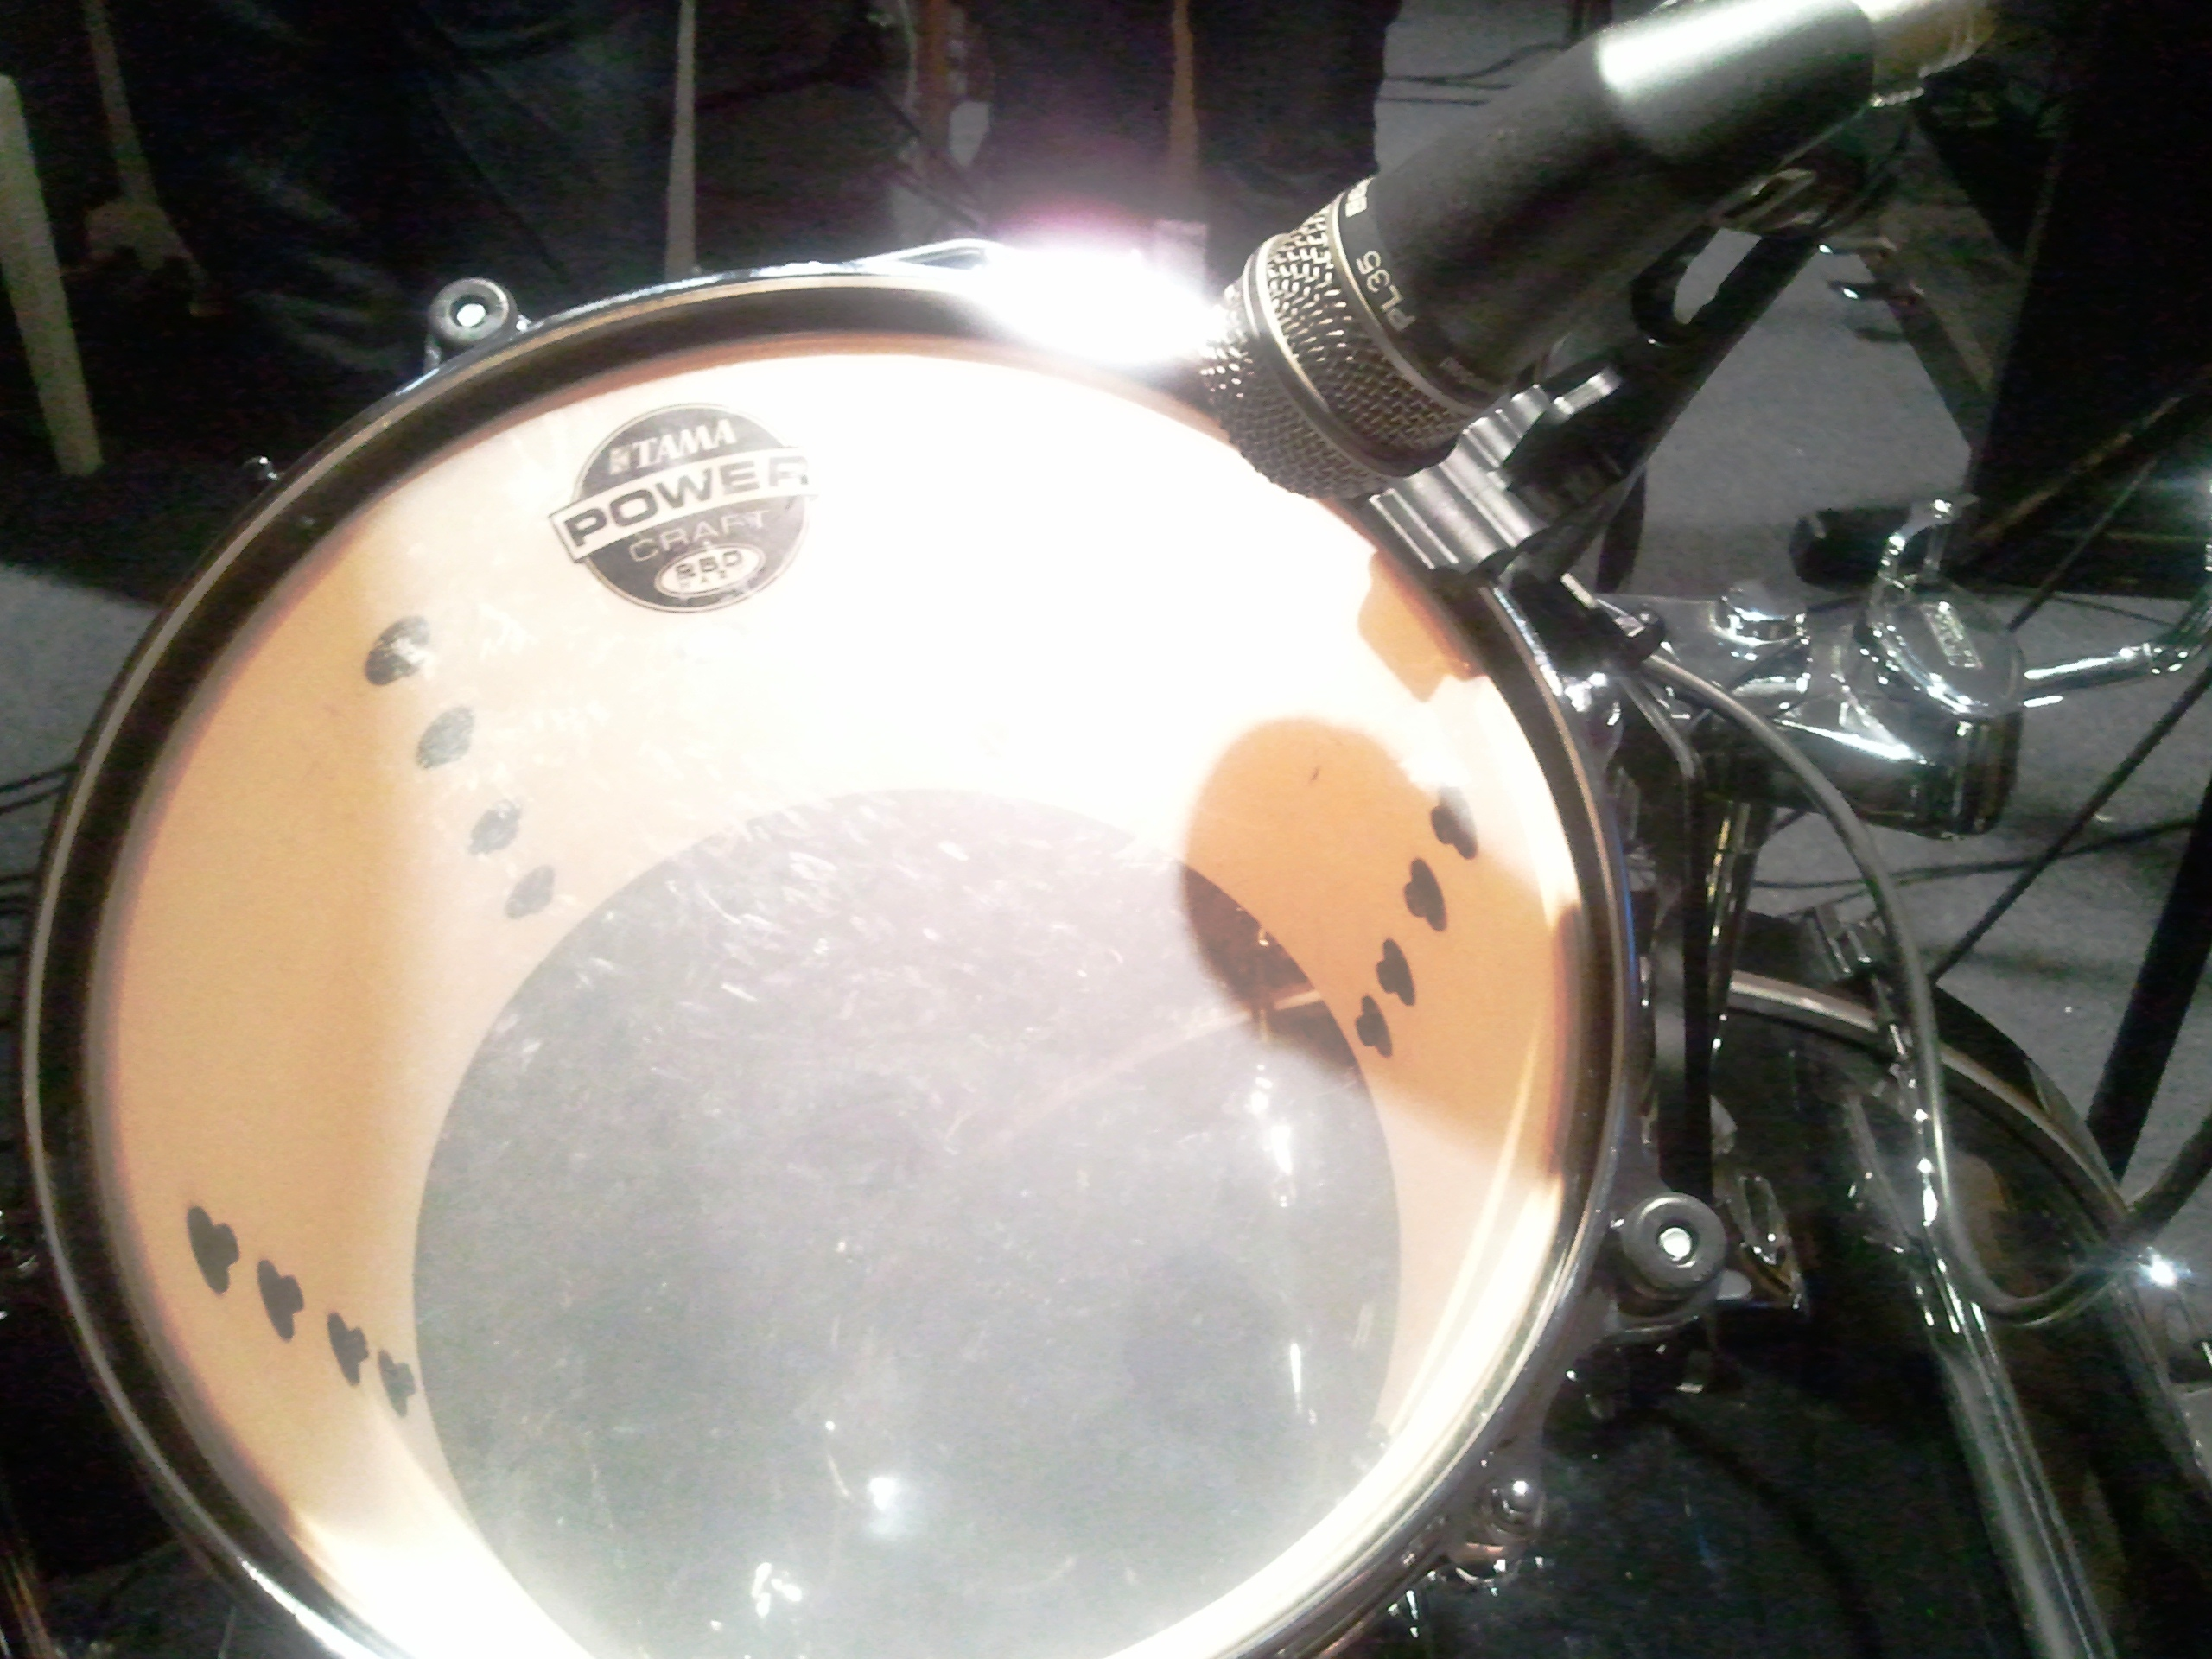
\includegraphics[width=0.8\textwidth]{drums} 
                % Bilddatei aus dem Unterverzeichnis bilder holen, skalieren auf 0.8*Satzspiegel
                \caption{Abnahme einer Trommel mit speziellem Anklemm-Mikrofon}\label{trommelmik}
                \end{figure}
            %------------- BILD ENDE ---------------
    
            %----------- BILD ANFANG -------------
            \begin{figure}[htp]     % h=here, t=top, b=bottom, p=page
                \centering
                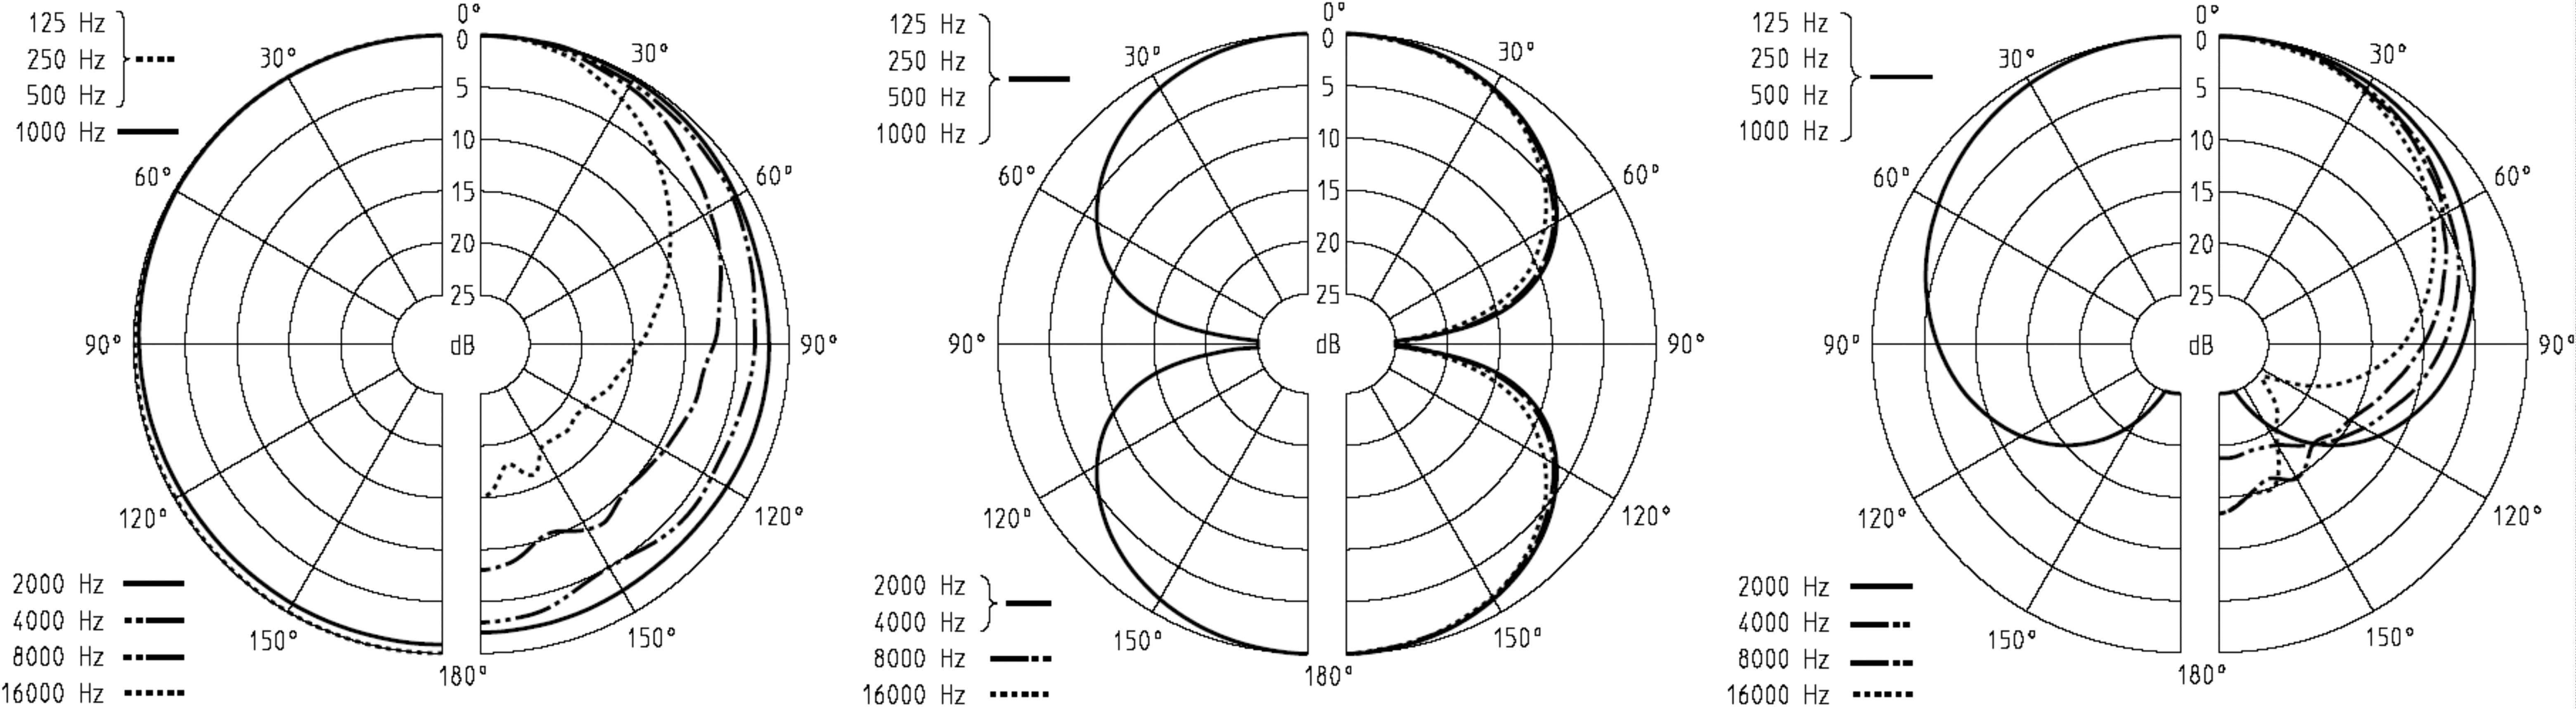
\includegraphics[width=1.0\textwidth]{3x_richtchars}
                \caption[Richtcharakteristiken von Kleinmembran-Studiomikrofonen]{Richtcharakteristiken von Kleinmembran-Studiomikrofonen. V.l.n.r.: Kugel, Acht, Niere. Die Bildbreite ist hier skaliert auf die volle Breite des Satzspiegels.}\label{richtch}
                % bei langen Bildunterschriften kann der optionale Parameter des caption-Befehls so wie hier fxr die Kurzfassung im Abbildungsverzeichnis genutzt werden  
                \end{figure}
            %------------- BILD ENDE ---------------  

        \section{Unterkapitel mit Mathematik, Bildern und Querverweisen}

            Für Formelsatz stellt \LaTeX\ die nummerierte Umgebung equation und die nicht-nummerierte Umgebung displaymath zur Verfügung. Mit label und ref kann dann im Text Bezug auf die Gleichungen genommen werden (Gleichung \ref{gl_fourier}). 

            \begin{equation}\label{gl_fourier}
            S(f) = \int_{-\infty}^{\infty} s(t)e^{-j 2 \pi f t}dt
            \end{equation}

            Mathematik im Zeilenmodus sieht so aus $f_0 = \frac{1}{2\pi} \sqrt{\frac{s}{m}}$, wxhrend dieselbe Gleichung als abgesetzte Formel -- hier mit der displaymath-Umgebung -- so aussieht: 

            \begin{displaymath}
            f_0 = \frac{1}{2\pi} \sqrt{\frac{s}{m}} 
            \end{displaymath}

            Fxr mehrzeilige Herleitungen oder Berechnungen benutzt man in \LaTeX\ die Umgebung eqnarray.

            Einheiten innerhalb von Formeln werden -- wie auch Text -- grundsxtzlich steil (nicht-kursiv) gesetzt. Innerhalb der mathematischen Umgebung nimmt man dafxr eine mbox (make box); die Abstxnde werden mit Komma, Semikolon oder quad eingestellt:

            \begin{displaymath}
            f_0 = \frac{1}{2\pi} \sqrt{\frac{s}{m}} \quad \mbox{[Hz]}
            % \, kleiner Abstand \; mittlerer Abstand \quad groxer Abstand
            \end{displaymath}

            Gleiches gilt fxr Funktionsnamen (sin, cos, arctan, log, ...). Fxr die meisten Funktionsnamen gibt es aber zur Vereinfachung entsprechende Befehle, sodass man nicht immer die mbox braucht.


        \section{Unterkapitel mit zwei Zitaten}

            Das wxrtliche Zitat wird durch Kursivschrift und Anfxhrungszeichen kenntlich gemacht, und natxrlich kommt ein Quellenverweis dazu:

            % \emph = Texthervorhebung durch Schriftumschaltung (emphasize), \medskip: vertikaler Abstand (\smallskip, \bigskip)
            \medskip
            \emph{Nisi irure excepteur eiusmod reprehenderit commodo ipsum exercitation.}
            \medskip

            Alternativ kann man ein Zitat auch in den laufenden Text einflechten, denn wie schon Sowodniok bemerkte, muss sich 
            \emph{Laboris tempor pariatur cillum sunt veniam labore duis ipsum eu cupidatat enim id.}
            Die Quellenverweise werden weiter unten erklxrt.


    \chapter{Ein anderes Kapitel}
                
        \section{Unterkapitel mit Fuxnote, Aufzxhlungen und Tabellen}\label{sec_fussnot}
                
            Fuxnoten sollte man sparsam und bewusst verwenden, erklxrende Zusxtze und Quellenverweise mxglichst in den Text integrieren. Damit bleiben Fuxnoten v.A. reserviert fxr wenige Ergxnzungen, die den Lesefluss stxren wxrden, aber nicht weggelassen werden sollen\footnote{Und so sieht die Fuxnote dann aus}.

            Fxr Aufzxhlungen stellt \LaTeX\ die beiden Umgebungen itemize und enumerate zur Verfxgung. So sieht eine itemize-Aufzxhlung aus:

            \begin{itemize}\setlength{\itemsep}{0ex} % itemsep ist der Abstand zwischen den Punkten der Aufzxhlung
                \item erster Punkt
                \item zweiter Punkt
            \end{itemize}

            Und das ist eine enumerate-Aufzxhlung:

            \begin{enumerate}\setlength{\itemsep}{0ex}
                \item erster Punkt
                \item zweiter Punkt
            \end{enumerate}

            Aufzxhlungen kxnnen auch verschachtelt werden. Als Beispiel dient hier eine enumerate-Umgebung innerhalb einer enumerate-Umgebung:

            \begin{enumerate}\setlength{\itemsep}{0ex}
                \item erster Punkt
                \item 
                    \begin{enumerate}\setlength{\itemsep}{-0.5ex}
                    \item erster Unterpunkt im zweiten Punkt
                    \item zweiter Unterpunkt im zweiten Punkt
                    \item dritter Unterpunkt im zweiten Punkt
                    \end{enumerate}
                \item dritter Punkt
            \end{enumerate}

            Als nxchstes folgt ein Beispiel fxr eine einfache Tabelle. Wie auch die Bilder mxssen die Tabellen stets Unterschrift und Nummer und zwingend einen Verweis im Text haben. In \LaTeX\ wird das wie bei den Abbildungen durch den caption-Befehl und das Befehlspaar label und ref gelxst (Tabelle \ref{t_buli}). Fxr ein modernes Tabellenlayout wird das \LaTeX-booktabs-Paket benutzt (siehe dazu die Kommentare im Quelltext). Die mittlere Spalte ist hier auf feste Breite (6 cm) gesetzt, damit bei viel Text ein automatischer Umbruch erfolgen kann.

            %----------- TABELLE START -------------
            \begin{table}[htp] 
                \centering
                \begin{tabular}{r|p{6cm}|c|c}  % Spalten nach Ausrichtung: l, c, r, p{breite}, mit zwei vertikalen Spaltentrennern
                    %bitte nicht das kleine L "l" und den Vertikalstrich "|" verwechseln!!! :)
                    % kleines L steht fxr eine linksbxndige Spalte, Vertikalstrich erzeugt eine Trennlinie zwischen zwei Spalten
                    \toprule
                    \multicolumn{4}{c}{\large\bfseries Erste Bundesliga, Spielzeit 2011/2012}\\ \midrule
                        Platz & Verein & TD & Punkte\\ \midrule
                        1 & Borussia Dortmund & +20 & 29\\ \midrule
                        2 & Borussia Mxnchengladbach & +14 & 29\\ \midrule
                        3 & FC Bayern Mxnchen & +26 & 28\\ \midrule
                        10 & Hertha BSC Berlin (Ballsportclub), Verein aus der Hauptstadt & $-$1 & 18 \\
                    \bottomrule
                \end{tabular}
                \caption{Bundesligatabelle vom 14. Spieltag}\label{t_buli}
            \end{table}
            %--------- TABELLE ENDE ---------------

            Tabelle \ref{t_buli2} zeigt eine Variante die ein kompakteres und eleganteres Ergebnis liefert, ohne vertikale Striche, dafxr mit eingefxrbten Zeilen.

            %----------- TABELLE START -------------
            \begin{table}[htp] 
                \rowcolors{1}{}{lgray} % bei jeder Zeile die Farbe wechseln, abwechselnd nix und hellgrau
                \centering
                \begin{tabular}{rlcc}  % Spalten nach Ausrichtung: l, c, r, p{breite} 
                    \toprule
                    \multicolumn{4}{c}{\large\sffamily Erste Bundesliga, Spielzeit 2011/2012}\\ \midrule
                        1 & Borussia Dortmund & +20 & 29\\ 
                        2 & Borussia Mxnchengladbach & +14 & 29\\
                        3 & FC Bayern Mxnchen & +26 & 28\\
                        10 & Hertha BSC Berlin & $-$1 & 18 \\ \bottomrule
                \end{tabular}
                \caption{Noch eine Bundesligatabelle vom 14. Spieltag}\label{t_buli2}
            \end{table}
            %--------- TABELLE ENDE ---------------

        \section{Unterkapitel mit drei exemplarischen Quellenverweisen}

            Quellenverweise werden mit Autorennamen und Jahr in runden Klammern gesetzt. Dazu wird hier das \LaTeX-natbib-Paket genutzt; der citep-Befehl erzeugt die Quellenangabe auf Basis der Eintrxge im Literaturverzeichnis. Auf gleiche Weise lassen sich auch mehrere Quellen zusammenfassen

            Auf Bxcher oder andere umfangreichere Quellen soll mit Seitenangabe verwiesen werden. Dafxr stellt der Befehle citep  einen optionalen Parameter zur Verfxgung. Und so sieht dann die vollstxndige Quellenangabe aus

            Die Quellen sollen im Literaturverzeichnis alphabetisch sortiert sein.


            \subsection{Unter-Unterkapitel zu Hyperlinks und Internetquellen}

                Die Beispiele unten im Literaturverzeichnis zeigen exemplarisch, welche Angaben zu den Quellen erforderlich sind (siehe dazu auch die Kommentare im \LaTeX-Quelltext). 

                Und noch eine \LaTeX-Spezialitxt zum Schluss: Durch die Einbindung von url- und hyperref-Paket im header werden die Quellenverweise im PDF-Dokument automatisch mit der jeweiligen Quelle im Literaturverzeichnis verlinkt, und bei Internetquellen werden die URLs anklickbar. Zudem werden die Verzeichnisse (Inhaltsverzeichnis, Abbildungs- und Tabellenverzeichnis) mit den jeweiligen Objekten verlinkt, und es werden Links zwischen jedem \emph{label} und  dazugehxrigem \emph{ref} erzeugt, also z.B. zwischen Bildverweis im Text und dem Bild. Die Farben der Links kxnnen im header frei eingestellt werden. Im hier vorgeschlagenen Layout sind die URLs und die Quellenverweise Dunkelblau, die anderen Links sind nicht hervorgehoben (Schwarz). 


    \chapter{Ergebnisse}

        Der thematische Teil schliext mit einer klaren inhaltlichen, auf der Grundidee aufbauenden thematischen Zusammenfassung, insbesondere bezogen auf die in der Arbeit gewonnenen eigenen Erkenntnisse und deren mxgliche Auswirkungen auf Forschung und Wissenschaft. 

        Ganz am Schluss, nach eventuellen Anhxngen, nach Abbildungs- und evtl. Tabellenverzeichnis, und nach dem Literaturverzeichnis, folgt die Eigenstxndigkeitserklxrung, die unterschrieben werden muss.

    \appendix

        \chapter{Material}

            \section{Fragebxgen, Messprotokolle etc.}

                In den Anhxngen landen ggf. Listings, Fragebxgen, Datenblxtter, Messprotokolle, Skizzen zu Versuchsaufbauten und xhnliches Material zur Arbeit. Im \LaTeX-Dokument leitet der Befehl appendix die Anhxnge ein.

        %--------------------- VERZEICHNISSE ----------------

        \listoffigures % Abbildungsverzeichnis erzeugen
        \listoftables % Tabellenverzeichnis erzeugen

    %--------------------- LITERATURLISTE ---------------
    % Die Einträge sollen alphabetisch sortiert sein.

    \bibliography{references} 
    \bibliographystyle{unsrtnat}

    %--------------------- EIGENSTÄNDIGKEITSERKLÄRUNG ---------------
    \clearpage\thispagestyle{empty}
    \eigen  % im header definiert
    %--------------------------------------- ENDE ------------------------------------

\end{document}